% !TEX root = trkjet.tex

The analysis procedure is similar to the procedure in \cite{PhysRevC.98.024908} with the additional requirement of being done differentially in \rvar. Measured tracks are associated with a reconstructed jet if they fall within $\Delta R < 0.8$ of the jet axis and are constructed as:

\begin{eqnarray}
\dfrac{\fd^{2} \nchmeas }{ \fd \pttrk \fd r} = \frac{1}{\varepsilon(\pttrk,\etatrk)} \frac{\Delta \Nch( \pttrk, r)}{ \Delta\pttrk \Delta r}
\end{eqnarray}

where $\Delta \Nch (\pttrk, r)$ represents the number of tracks within a given \pttrk\ and $r$ range. The efficiency correction is applied as a $1/\varepsilon(\pttrk,\etatrk)$ weight on a track-by-track basis, assuming $\pttrk = \pTtrue$. While that assumption is not strictly valid, the efficiency varies sufficiently slowly with $\pTtrue$ that the error
introduced by this assumption is less than 1\%.

The measured track yields need to be corrected for the underlying event and fakes from the soft processes. In \pp\ collisions, the UE contribution is negligible due to minimal pileup and the fake subtraction is done by estimating fake rates from the MC samples using tracks that do not have an associated truth match. For \pbpb\ collisions, the fakes and UE are estimated together in a two step process: first, MC overlay events reweighed to match the centrality distribution in jet triggered data are used to generate $\eta-\phi$ maps of the average number of particles in a given annulus around a jet. This is done for tracks without a truth match and as a function of \ptjet, \etajet, \phijet, angle of the jet to the reaction plane\footnote{The reaction plane angle $\Psi$ is determined on an event-by-event basis by a standard method using the $\phi$ variation of transverse energy in the forward calorimeter \cite{ATLAS:2012at}} $ \mathrm{d}\Psi_{\mathrm{jet}}$, \rvar, \pt, and centrality. In the second step, the $\eta-\phi$ maps are convoluted with $\eta_{\mathrm{jet}}$, $\phi_{\mathrm{jet}}$, and $\mathrm{d}\Psi_{\mathrm{jet}}$ distributions in the jet triggered data to estimate the yields of charged particles for the jet under study, \mbox{$\fd^2 \nch^{\mathrm{UE+Fake}}(r) / \fd \pttrk \fd r|_{\mathrm{cent}}$}. The yields are independent of the angular distance $r$, decrease with the decreasing collision centrality, increasing \pttrk, and increasing azimuthal distance to the second-order event plane. 

\begin{align}
\frac{\fd^2 \nchsub }{ \fd \pttrk \fd r } &=  \frac{\fd^2 \nchmeas }{ \fd \pttrk \fd r} -  \frac{ \fd^2 \nch^{\mathrm{UE+Fake}}(r)  }{ \fd \pttrk \fd r} 
\end{align}

Figure~\ref{fig:UEsize} shows the charged-particle distributions prior to the UE and fake track subtraction, $ \fd^2 \nchmeas / \fd \pttrk \fd r$, divided by the distributions after the subtraction, $ \fd^2 \nchsub / \fd \pttrk \fd r $ as a function of \rvar\ for different \pttrk\ intervals and $126 < \ptjet < 158$ \GeV for six centrality selections. The UE is the highest for 1.0~\GeV\ charged particles at large values of \rvar\ and in central collisions for \ptjet\ between 126--158~\GeV, with the signal to background being approximately 1:100. It is rapidly decreasing towards more peripheral collisions, larger \pttrk\ and smaller \rvar. Furthermore, the ratio slowly decreases with increasing \ptjet.

\begin{figure}
\centerline{
 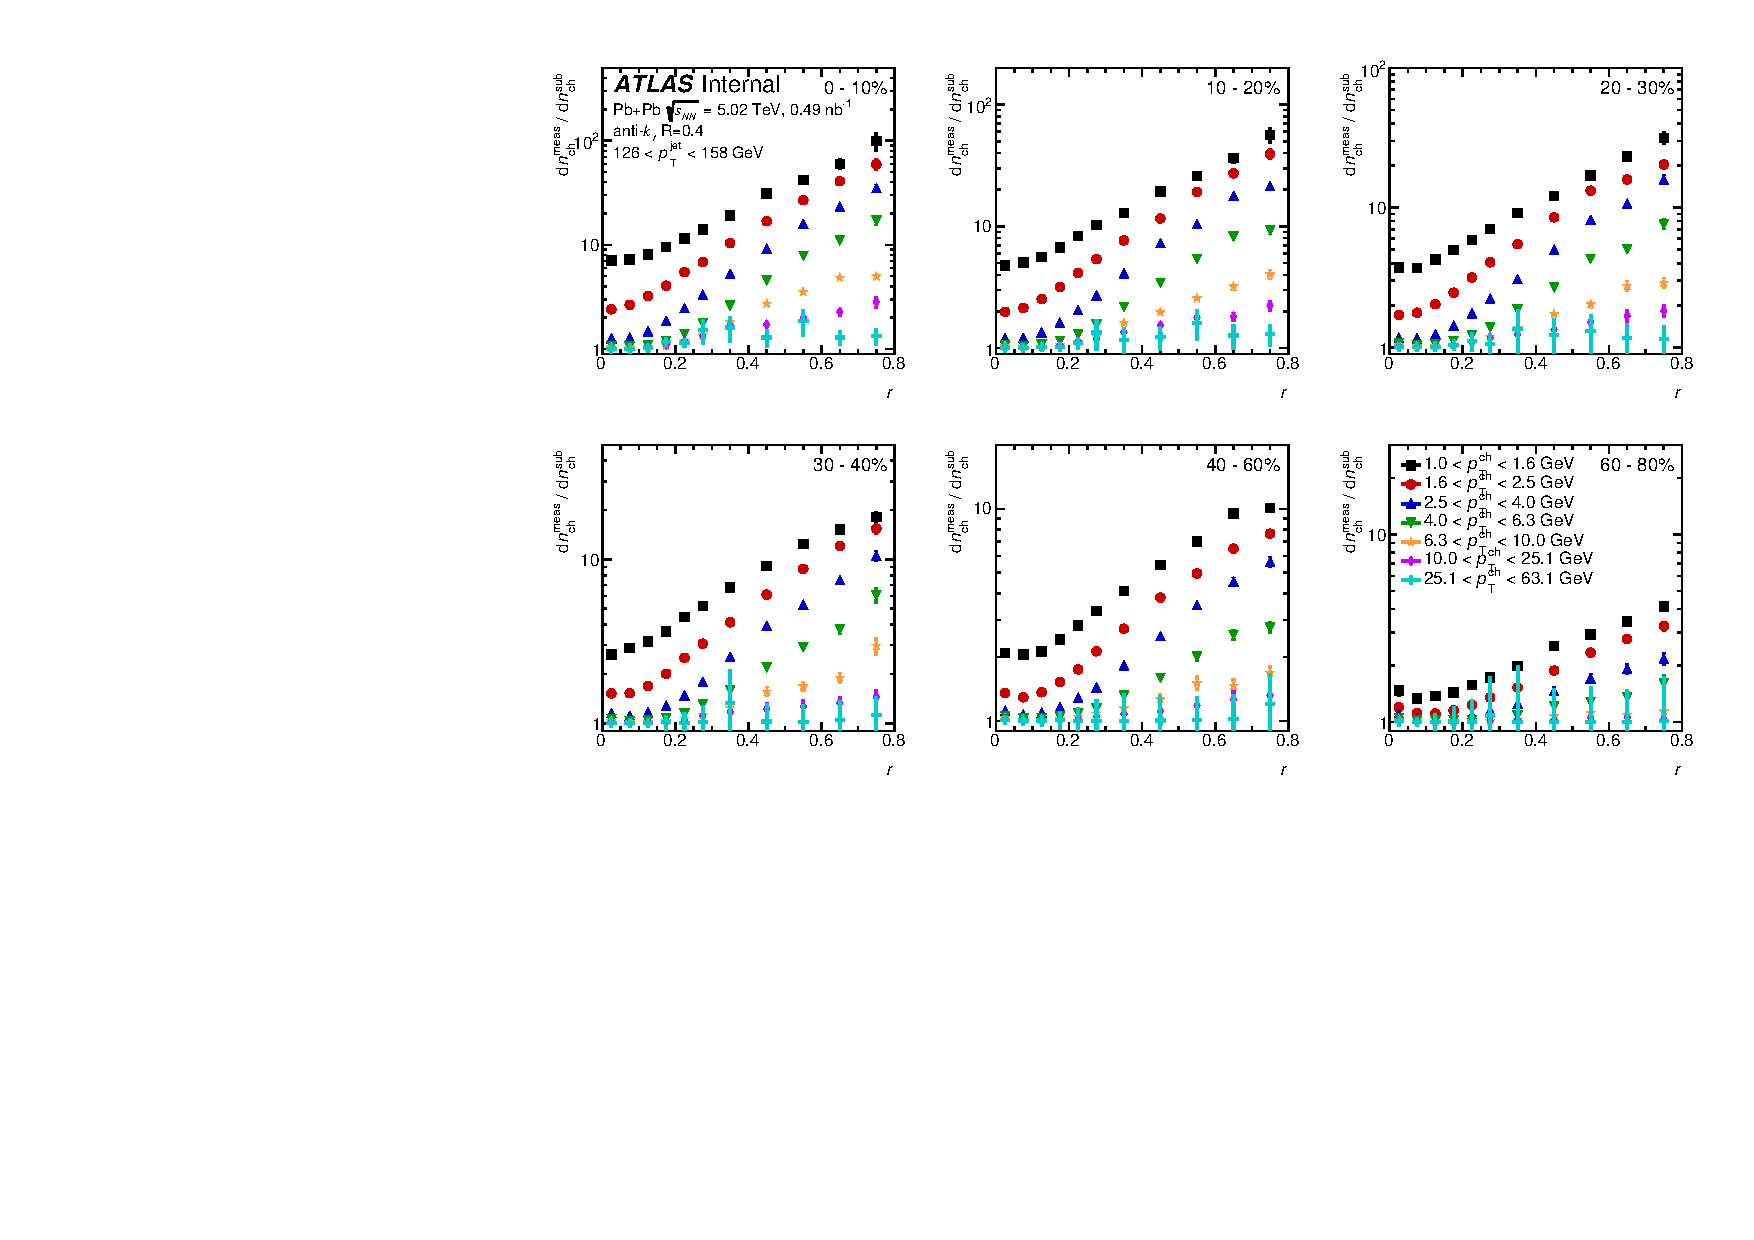
\includegraphics[width=0.95\textwidth]{figures/performance/UE_B2S_single_0.pdf} }
\caption{ Ratio of the raw charged particle distributions to those after the subtraction of the UE and fake tracks as a function of \rvar\ for different \pttrk\ intervals, six centrality selections and for \ptjet\ between 126--158~\GeV.}
\label{fig:UEsize}
\end{figure}

The intrinsic underlying event from the hard scattering process is not subtracted in both \pp\ and \pbpb\ collisions because this would be generator dependent and make comparisons between the two systems non-trivial. 

%The fraction of fake tracks is found to be below 2\% of the tracks that pass the selection in all track and jet kinematic regions in this analysis.

To remove the effects of the bin migration due to the jet energy and track-momentum resolution, the subtracted $\fd^2 \nchsub /\fd\pttrk \fd r$ distributions are corrected by a two-dimensional Bayesian unfolding~\cite{DAgostini:1994zf}
in \pttrk\ and \ptjet\ as implemented in the RooUnfold package~\cite{Adye:2011gm}.  
Two-dimensional unfolding is used because the calorimetric jet energy response depends on the fragmentation pattern of the jet~\cite{Aad:2011he}.
Four-dimensional response matrices are created from the \pp\ and \pbpb\ MC samples using the generator-level and reconstructed \ptjet, and the generator-level and reconstructed charged-particle \pttrk. They are corrected for tracking efficiencies and are evaluated in bins of \rvar\ and centrality. The Bayesian procedure requires a choice in the number of iterations.
Additional iterations reduce the sensitivity to the choice of prior, but may
amplify statistical fluctuations in the distributions.
After four iterations the 
charged particle distributions are found to be stable for both the \PbPb\ and \pp\ data.
A separate one-dimensional Bayesian unfolding is used to correct the measured \ptjet\ spectra that are used to normalize the unfolded charged particle distributions.
To achieve better correspondence with the data, the response matrices for both the one and two dimensional unfolding are reweighed so that the distributions match the shapes in the reconstructed data.

An independent bin-by-bin unfolding procedure is also used to correct for migrations originating from the finite jet and track angular resolutions. Two corresponding \Dptr\ distributions are evaluated in MC samples, one using generator-level jets and primary particles and the other using reconstructed jets and charged particles with their reconstructed \pttrk\ replaced by generator-level transverse momentum, \pTtrue. The ratio of these two MC distributions provides a correction factor which is then applied to the data. 

The final particle-level corrected distributions, normalized by the area of the annulus under question are defined as:
\begin{eqnarray}
 \label{eq:Dpt}
   \Dptr = \frac{1}{N_\mathrm{jet}^\mathrm{unfolded}} \frac{1}{A(r)} \frac{\fd^2 \nchunf(r)}{\fd \pt \fd r},
 \end{eqnarray}
where $\text{N}_{\text{jet}}^{\text{unfolded}}$ is the unfolded number of jets in a given \ptjet\ interval.

The performance of the full analysis procedure is validated in the MC samples by comparing the fully corrected charged particle distributions to the generator-level distributions. Good closure (< 3\%) is seen for low \pt\ particles. Algorithmic effects from the jet reconstruction software in reconstructing high \pt\ particles near the jet edge lead to a larger non-closure in those regions of the measurement phase-space. The analysis is done where the non-closure in the \pp\ MC sample is less than 5\%, excluding the following regions of phase space: 6--10 GeV tracks above $\rvar > 0.3$, 10--25 GeV tracks above $\rvar > 0.3$, and 25--63 GeV tracks above $\rvar > 0.2$ for 126--158 GeV jets; 10--25 GeV tracks above $\rvar > 0.4$, and 25--63 GeV tracks above $\rvar > 0.3$ for 158--200 GeV jets; 25--63 GeV tracks above $\rvar > 0.3$ for 200--251 GeV jets.



